\documentclass[12pt]{article}

\usepackage[utf8]{inputenc}
\usepackage[brazil]{babel}
\usepackage[a4paper,left=3cm, right=2cm,top=2.5cm, bottom=2.5cm]{geometry}
\usepackage{amsmath}
\usepackage{graphicx}
\usepackage{float}
\usepackage{multirow}
\usepackage{authblk}
\usepackage{fancyhdr}
\usepackage{xcolor}

\title{\textbf{ENG1456 - Redes Neurais - Trabalho 1 Classificação}}
\author{\textbf{Aluno: Matheus Carneiro Nogueira - 1810764}}
\affil{}
\author{\textbf{Professora: Marley Velasco}}
\affil{}
\pagestyle{fancy}
\fancyhf{}
\lhead{{\small \textcolor{gray}{PUC-Rio ENG1456}}}
\renewcommand{\headrulewidth}{0pt}
\date{}
\renewcommand{\footrulewidth}{0pt}
\fancyfoot[C]{\thepage}

\begin{document}
	\maketitle
	\tableofcontents
	
\begin{abstract}
	Este documento consiste no relatório do trabalho 1 do módulo de Redes Neurais da disciplina ENG1456 da PUC-Rio. Nele será explicada a implementação de modelos de Redes Neurais MLP para a clafficicação do dataset Ionosphere, disponibilizado pela professora da disciplina e disponível em \cite{Dataset}. A seções do relatório são definidas de acordo com as perguntas principais que constam no arquivo Guia de Atividades.
\end{abstract}

\section{Apresentação do dataset}\label{sec:apresentacao}

Com o intuito de criar um modelo de rede neural para classificar o dataset \textit{Ionosphere}, é essencial que, antes de implementar a rede, estudemos o dataset em si. Como descrito no artigo \cite{Paper1989} e pelas informação disponibilizadas em \cite{Dataset}, este dataset consiste no sistema de radares da região de Goose Bay, Labrador, o qual possui 16 antenas de alta frequência. O alvo dessas antenas foram elétrons livres na Ionosfera e, bons retornos do radar consistem em retornos que indicam alguma estrutura na ionosfera, enquanto mals retornos são aqueles cujo sinal passa livre pela Ionosfera e não retorna. É justamente esta classificação que a Rede Neural desenvolvida neste trabalho almeja realizar, separar as entradas em "good" ou "bad". Com isso, notamos que a rede pode possuir um único neurônio de saída, que mapeia 0 em "bad" e 1 em "good".

\section{Compreensão do problema e análise de variáveis}

\subsection{Observe a base de dados do problema. Existem variáveis que podem ser	eliminadas do dataset? Justifique.}\label{subsec:eliminadas}

Ao analisar as colunas do dataset, percebe-se que as duas primeiras colunas, \textit{info\_1} e \textit{info\_2} aparentam ser colunas inteiramente de 1 e 0, respectivamente. Para ter certeza, uma vez que observar apenas o head e tail não é suficiente, as colunas inteiras foram analisadas e confirmou-se que a segunda coluna, \textit{info\_1} de fato é inteiramente de 0. Sendo assim, é recomendável que ela seja excluída do dataset pois, além de não trazer nenhuma informação útil à classificação dos retornos de rádio, essa informação pode atrapalhar o treinamento da rede, uma vez que ambos os retornos bons e ruins apresentam valor 0 neste atributo.

\subsection{Implemente técnicas de visualização de dados e seleção de variáveis para extrair características importantes sobre a base de dados. Explique	a motivação destas técnicas e o que é possível inferir dos resultadosobtidos.}


Foi utilizado o \textit{pairplot} da biblioteca seaborn para visualizar os valores das entradas de nossa rede neural com o intuito de procurar alguma informação útil, tanto para a compreensão da base de dados, quanto para a modelagem da rede neural. Serão adicionadas apenas as imagens úteis para alguma interpretação, com o intuito de não poluir desnecessariamente este relatório.

Como pode ser visto na imagem abaixo, figura \ref{fig:pairplot0a7}, os retornos classificados como bons parecem possuir alguma relação com os valores maiores ou iguais a zero nas colunas info\_2, info\_4 e info\_6. Esta informação é interessante pois, caso alguma entrada de teste possua, nestas colunas, valores maiores que zero, há uma chance maior de pertencerem à classe "good".

\begin{figure}[H]
	\centering
	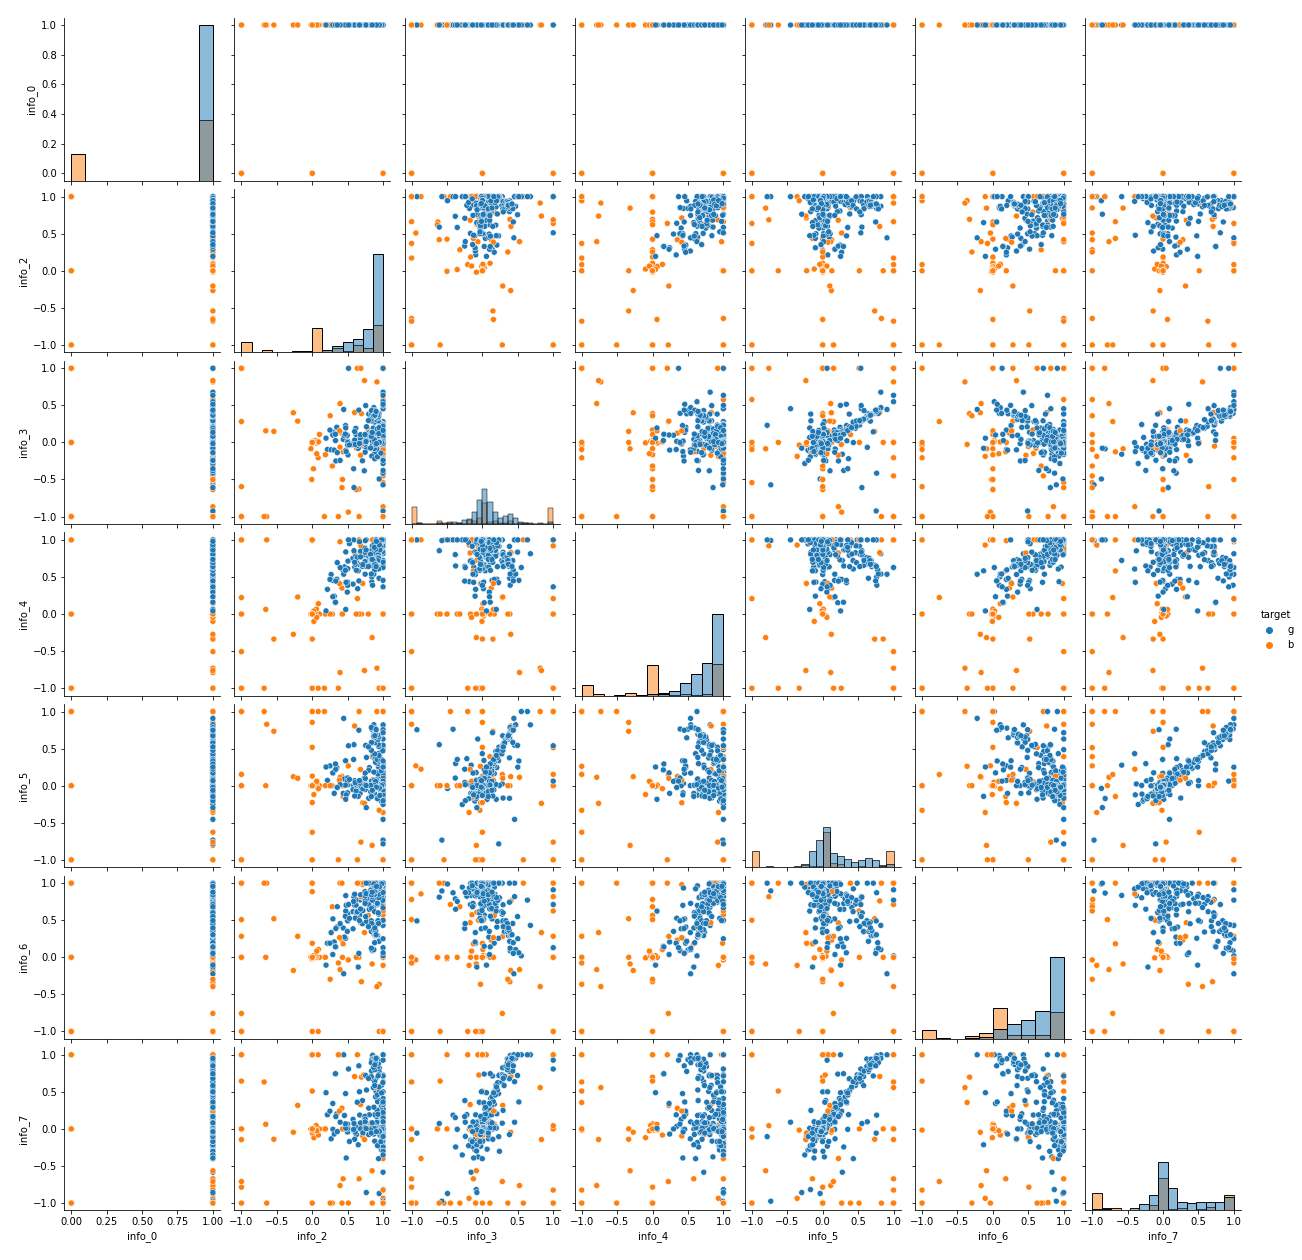
\includegraphics[width=1.1\linewidth]{../pairplot0a7}
	\caption{info\_0 a info\_7}
	\label{fig:pairplot0a7}
\end{figure}

Já a figura \ref{fig:pairplot21a28} parece revelar uma relação linear entre os retornos classificados como "good" ao olharmos as colunas info\_23, info\_24, info\_26 e info\_28. Isso pode indicar que, entradas que possuam estes valores próximos à uma determinada reta possuem maior probabilidade de serem da classe "good".

\begin{figure}[H]
	\centering
	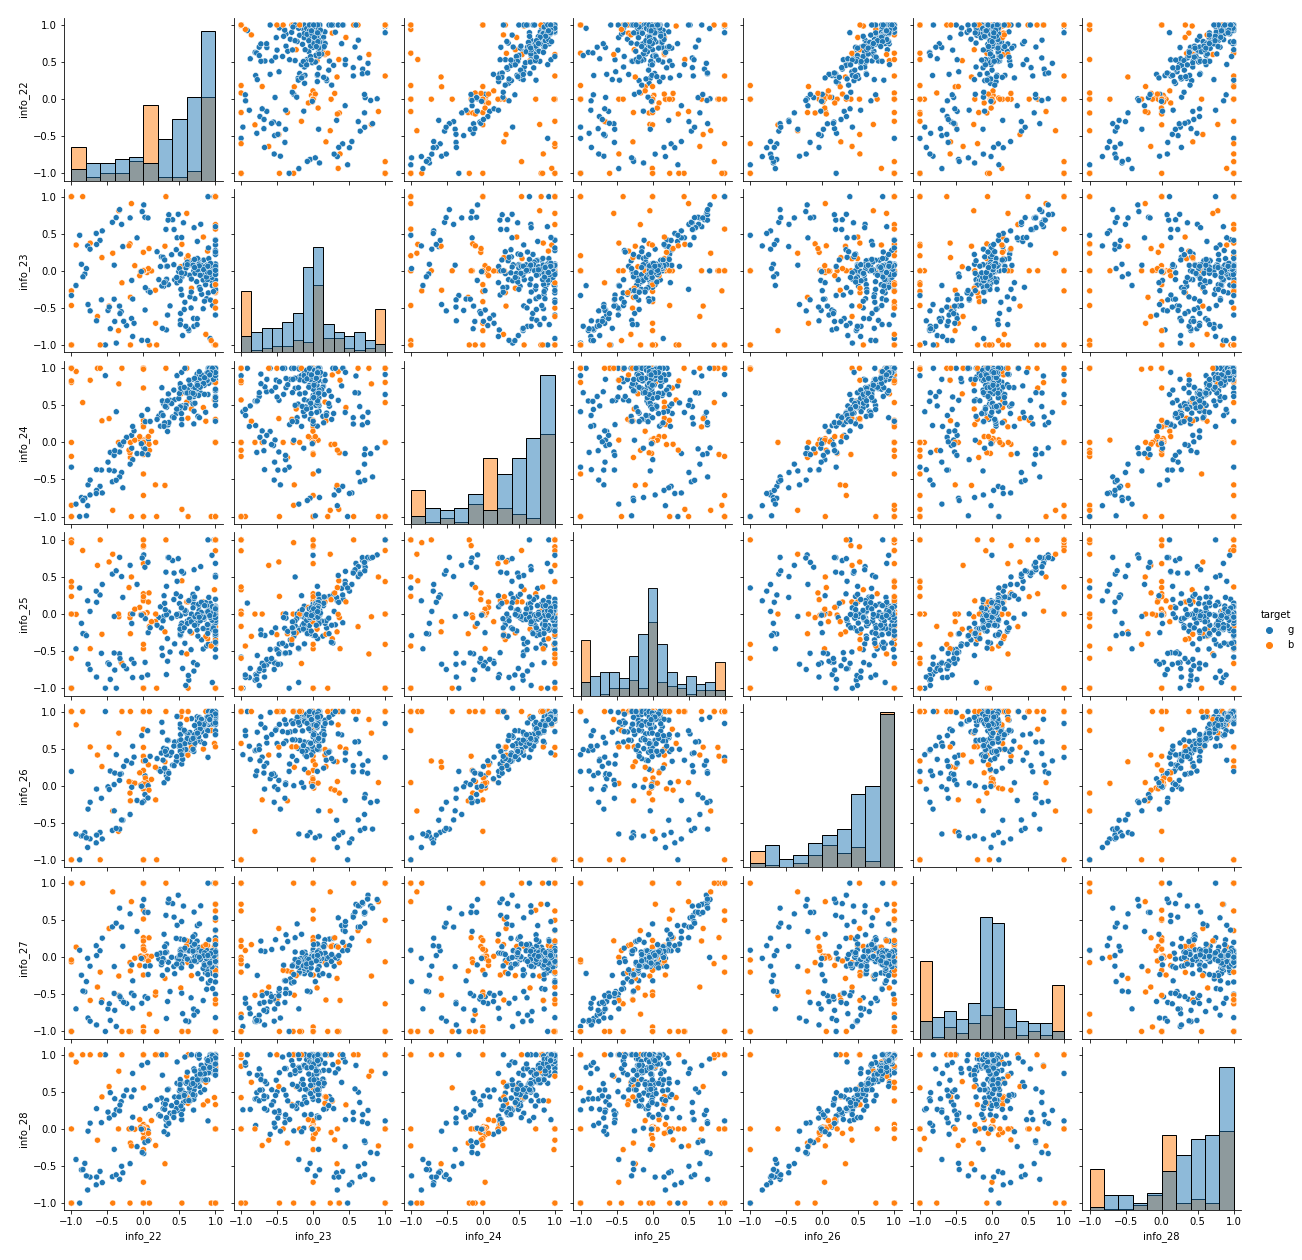
\includegraphics[width=1.1\linewidth]{../pairplot21a28}
	\caption{info\_21 a info\_28}
	\label{fig:pairplot21a28}
\end{figure}

Por fim, todas as imagens mostram que os retornos da classe "good", em azul, apresentam algum nível de concentração ou padrão, enquanto os retornos "bad" são aqueles mais dispersos ao longo de toda a escala de valores.

\section{Treinamento do modelo de Rede Neural}

\subsection{Com as configurações do modelo MLP previamente definidas no script, faça o treinamento da Rede Neural sem normalizar os atributos	numéricos. Comente o resultado obtido, baseado nas métricas de	avaliação disponíveis (acurácia, precision, recall, F1-Score, Matriz de	confusão, etc.)}

O nosso primeiro modelo de rede MLP foi criado de acordo com as especificações já presentes no script disponibilizado. Essa Rede Neural possui as seguintes especificações:

\begin{figure}[H]
	\centering
	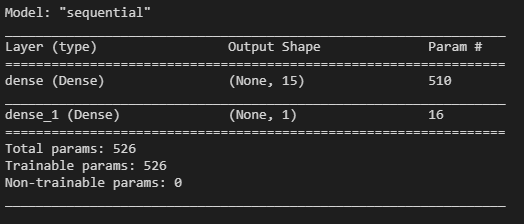
\includegraphics[width=0.7\linewidth]{Imagens/SumarioModeloNaoNormalziado}
	\caption{Sumário do Modelo MLP Não Normalizado}
	\label{fig:sumariomodelonaonormalziado}
\end{figure}

Como a figura \ref{fig:sumariomodelonaonormalziado} revela, nossa rede possui 1 camada escondida completamente conectada (densa) com 15 neurônios e a camada de saída com apenas 1 neurônio, como explicado na seção \ref{sec:apresentacao}. Além disso, nota-se que o número de parâmetros treináveis é 526. Essa informação será importante quando variarmos o número de épocas de treinamento, que neste caso é 50, uma vez que possuir épocas demais pode significar um overfiting de nosso modelo, gerando perda de generalização. 

Para analisar a acurácia deste modelo, observemos as figuras abaixo.

\begin{figure}[H]
	\centering
	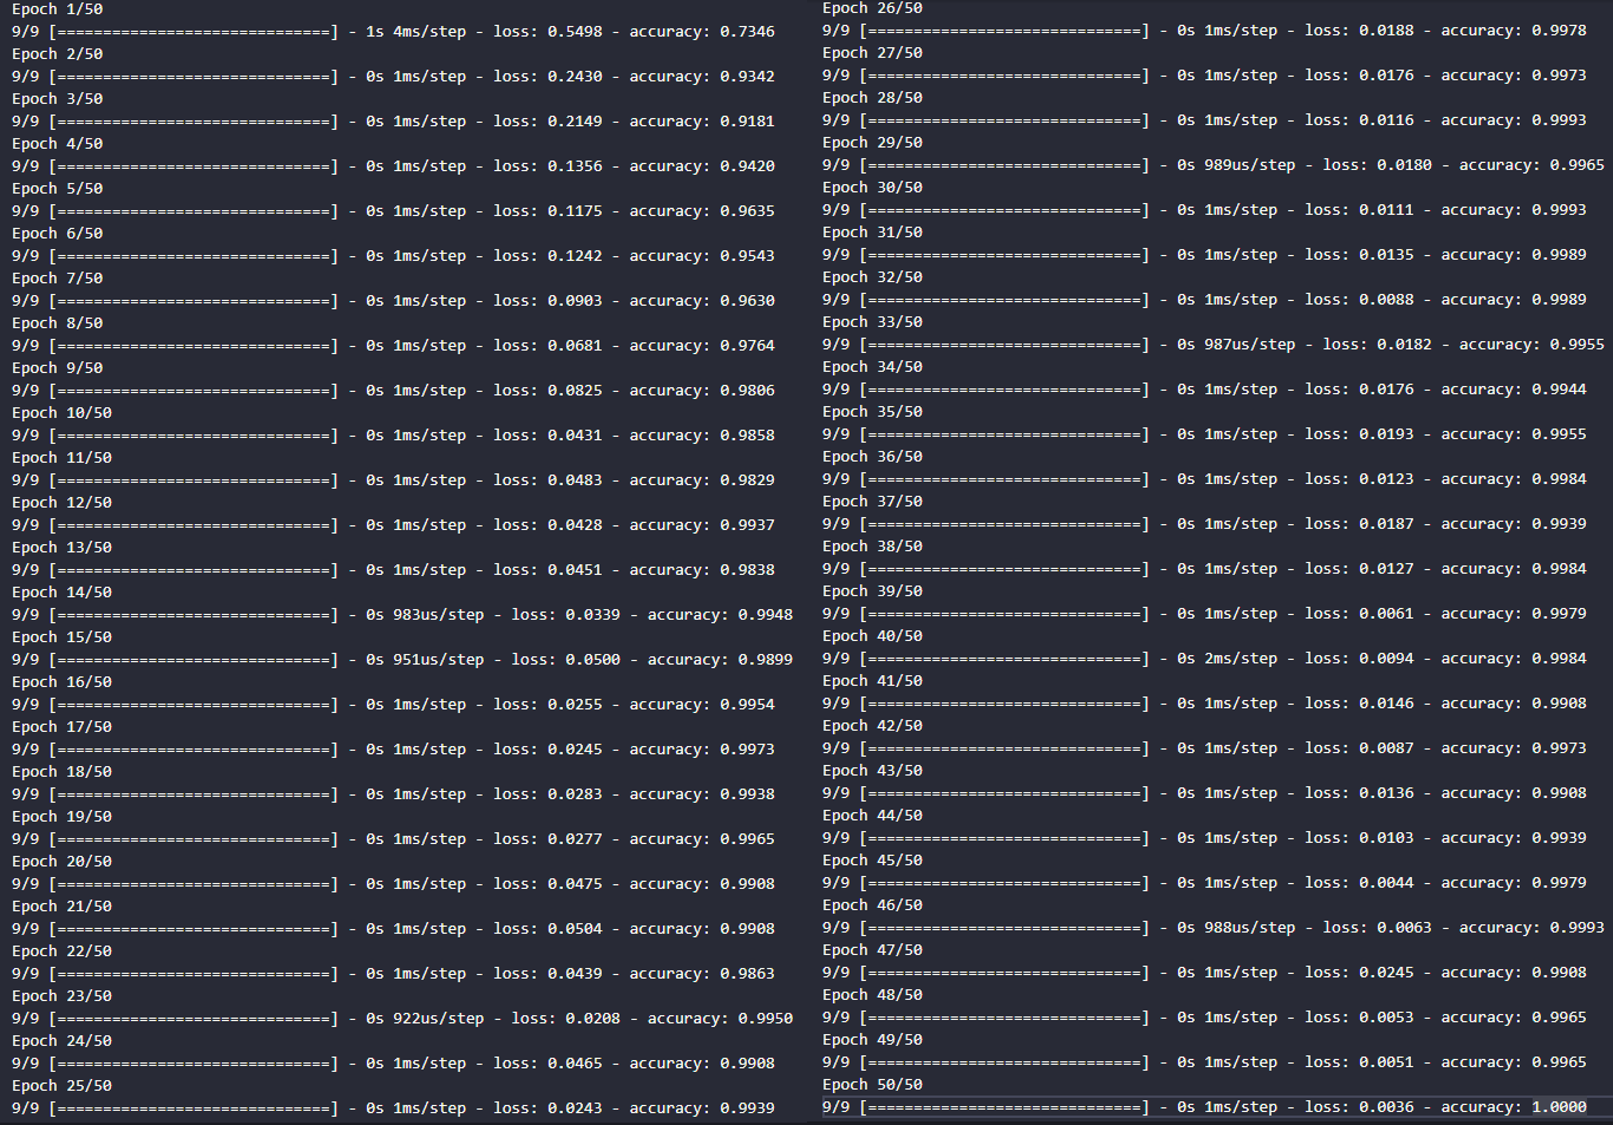
\includegraphics[width=1.1\linewidth]{Imagens/Fit_NaoNormalizado}
	\caption{Output do treinamento do modelo não normalizado}
	\label{fig:fitnaonormalizado}
\end{figure}

\begin{figure}[H]
	\centering
	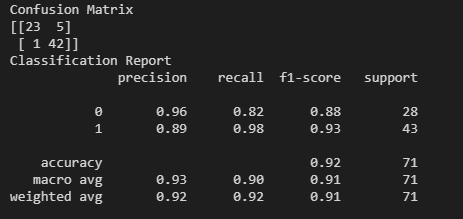
\includegraphics[width=0.7\linewidth]{Imagens/resultadoNaoNormalizado}
	\caption{Métricas do modelo não normalizado}
	\label{fig:resultadonaonormalizado}
\end{figure}

O modelo em questão apresentou acurácia de 92\%, o que, a priori, é bom, vide figura \ref{fig:resultadonaonormalizado}. Essa métrica indica que em 92\% dos casos apresentados na fase de validação a rede foi capaz de classificar corretamente o retorno como bom ou ruim. Podemos observar, também, que a evolução da acurácia do modelo na figura \ref{fig:fitnaonormalizado}. Percebe-se que, uma vez atingida a acurácia de 0.99 houve pouca flutuação nos valores dessa métrica, que na última época atingiu o valor de 1.00. Isso pode indicar que a quantidade de épocas não foi grande demais, pois, se fosse, veríamos uma queda maior na acurácia depois de certa época ou crescimento do valor de \textit{loss}. Novamente, apenas quando testarmos outros valores de época poderemos confirmar se este é um bom valor, mas, por hora, ele parece razoável. 

A precisão de nosso modelo foi de 0.96 para os casos zero, isto é, "bad" e de 0.89 para 1, "good". Isso nos mostra que a rede possui um grande desempenho em classificar corretamente os retornos ruins e um desempenho um pouco pior em classificar os retornos bons. Isso é curioso uma vez que a nossa base de treino foi composta de 189 entradas 1 e 98 entradas 0, o que mostra que nossos dados são razoavelmente desbalanceados. Uma solução possível para melhorar essa métrica é construir a base de treino de outra forma, garantindo maior equilíbrio entre os retornos bons e ruins. Para a situação deste dataset, podemos argumentar que é melhor a rede classificar um retorno bom como ruim do que um retorno ruim como bom, uma vez que este segundo erro poderia causar a utilização de uma antena defeituosa, o que é mais prejudicial que não utilizar uma antena em bom funcionamento. Sendo assim, a rede possuir uma precisão maior para os retornos ruins é melhor do que o caso contrário, se ela apresentasse precisão menor para retornos ruins.

A métrica recall indica quanto a rede acertou a classificação de uma entrada da classe 0, por exemplo, em relação ao número de entradas da classe 0. É justamente o recall que nós podemos observar na matriz de confusão da figura \ref{fig:resultadonaonormalizado}. Nosso resultado indica que, em 82\% dos casos em que o retorno era ruim, nosso modelo acertou que ele era ruim e, em 98\% dos casos em que o retorno era bom, a rede  classificou corretamente que era bom. Esta métrica usada em conjunto com a precisão é útil para avaliar o quão preciso é nosso modelo em classificar corretamente as entradas em relação à classe correta da entrada. Como nossa precisão é maior para a classe "ruim" e o recall é menor para essa mesma classe, podemos ter maior confiança do que se ambas as métricas fossem maiores para uma classe específica, o que indicaria que nosso modelo não seria muito bom em classificar a entrada nesta classe.

Por fim, o F1-score  é a média harmônica entre a Precisão e o Recall. Uma vez que já foram analisadas as métricas recall e precisão, o f1-score não fornece, a priori, nenhuma nova informação importante. No entanto, ao alterar o modelo, utilizaremos a comparação dessa métrica para identificar melhoras na qualidade das redes.

A figura abaixo indica a matriz de confusão relativa de nosso modelo. Como nós já comentamos sobre ela e sobre a métrica Recall, aqui apenas consta um resumo de sua interpretação.
\begin{figure}[H]
	\centering
	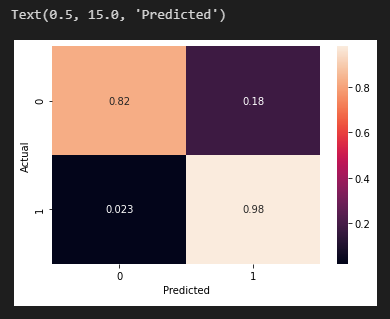
\includegraphics[width=0.5\linewidth]{Imagens/ConfusionMatrizNaoNormalizado}
	\caption{82\% das entradas ruins foram classificadas como ruins e 98\% das boas foram classificadas como boas}
	\label{fig:confusionmatriznaonormalizado}
\end{figure}




\subsection{Agora normalize os dados de entrada e treine novamente o modelo MLP.	Avalie os resultados obtidos e comente o efeito da normalização no	treinamento da Rede Neural.}\label{subsec:normalizada}
	
Realizar uma normalização dos dados de entrada é uma estratégia útil para tentar aumentar tanto a eficiência computacional quanto a precisão da classificação. A normalização é importante, também, para adequar os valores aos domínios das funções de ativação que, neste caso, são a \textit{ReLu} (Rectified Linear Activation Unit) utilizada para as camadas escondidas e a \textit{Sigmoid} para a camada de saída. Os valores originais já eram, de certo modo, normalizados, uma vez que todos estavam dentro do intervalo $[-1 1]$. Vejamos o que normalizar par ao intervalo $[0 1]$ fará com nossa rede.

Ao normalizar as entradas, novamente foi verificada a coluna \textit{info\_0}, que permaneceu na base de dados na seção \ref{subsec:eliminadas}. Ela permanece, obviamente, inalterada, uma vez que seus valores já eram 0 ou 1. No entanto, foi modelada uma rede com e outra sem esta coluna e não foi observada grande diferença de qualidade de classificação. Sendo assim, a coluna permanece na base de dados e os resultados para a rede sem esta coluna não serão exibidos.

Além de normalizar, nenhuma outra modificação foi feita no modelo, então podemos seguir para a explanação dos resultados. As figuras a seguir exibem o output do treinamento do modelo e as métricas dos resultados de teste.

\begin{figure}[H]
	\centering
	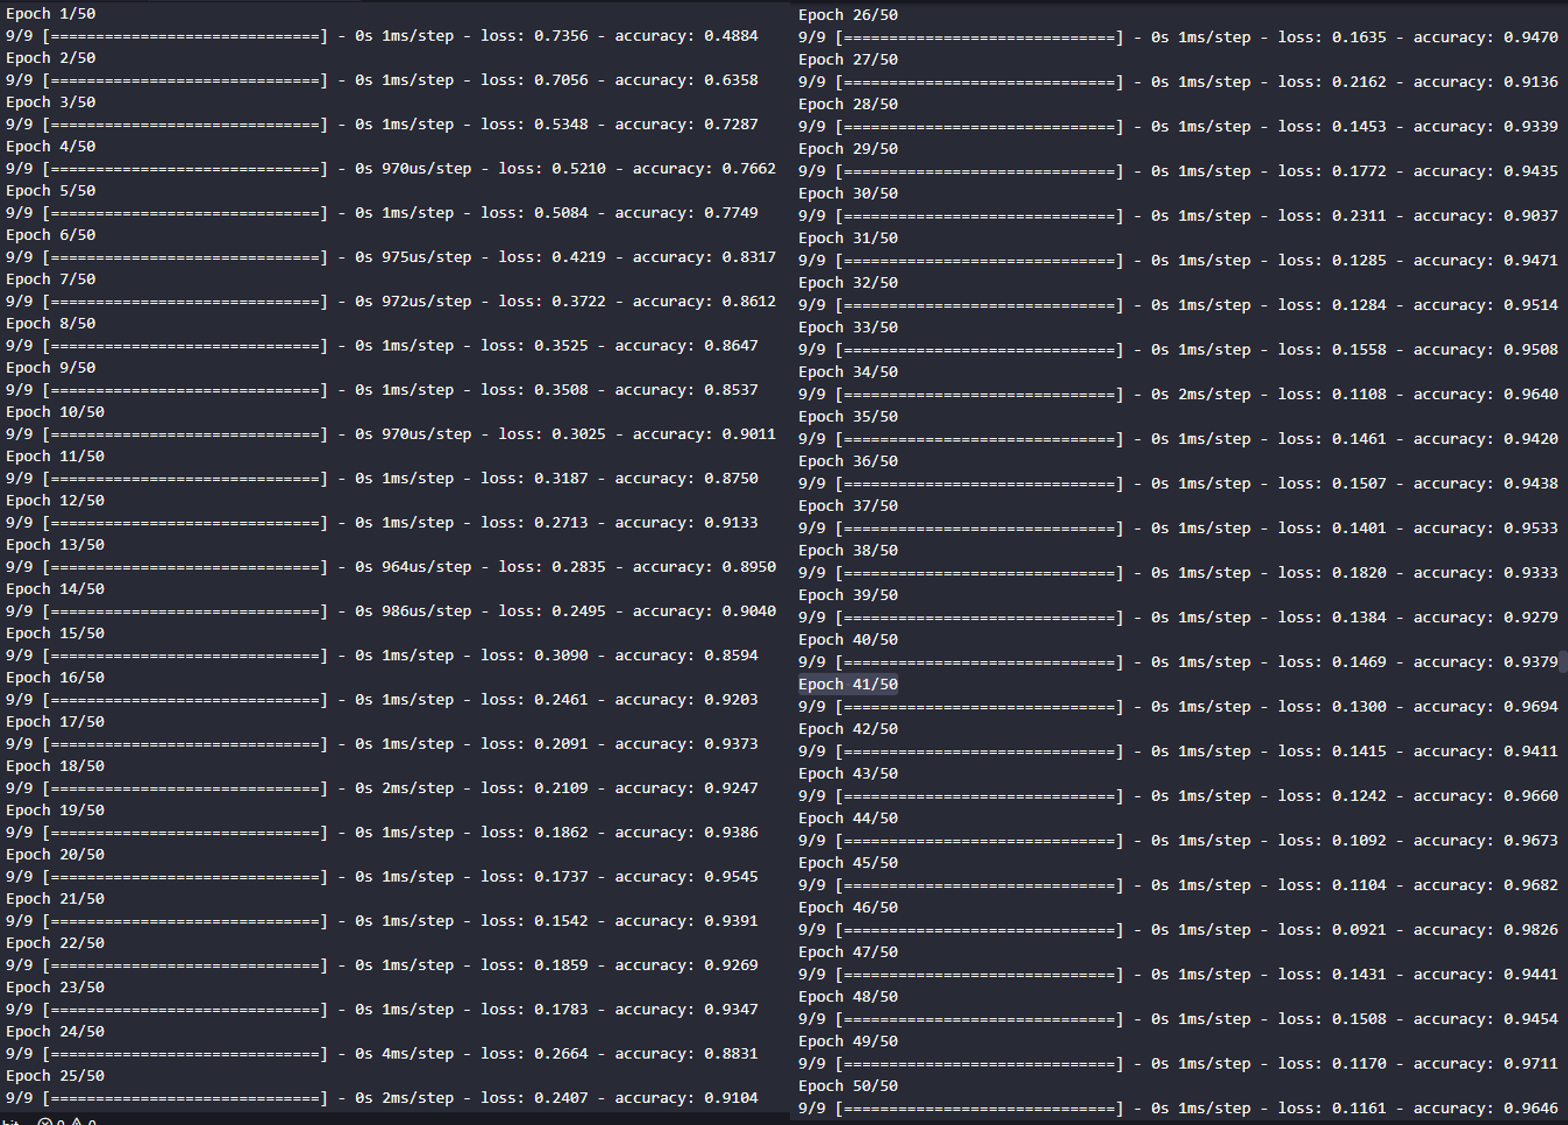
\includegraphics[width=1.1\linewidth]{Imagens/Fit_Normalizada}
	\caption{Output do treinamento do modelo normalizado}
	\label{fig:fitnormalizada}
\end{figure}
\begin{figure}[H]
	\centering
	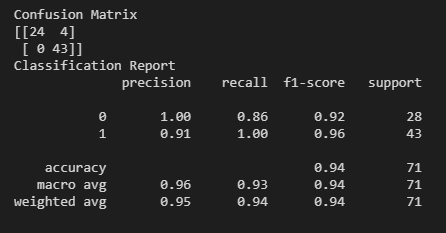
\includegraphics[width=0.7\linewidth]{Imagens/resultadoNormalizada}
	\caption{Métricas do modelo normalizado}
	\label{fig:resultadonormalizada}
\end{figure}

A acurácia do modelo normalizado é maior que a do modelo não normalizado. Obtivemos um aumento de 0.02 nesta métrica, passando de 0.92 para 0.94. Como nossa acurácia já possuía um valor alto, este aumento, por si só, pode não significar grandes melhorias gerais da qualidade da rede, então é importante analisarmos, novamente, as demais métricas. Além disso, ao analisar a evolução da acurácia na figura \ref{fig:fitnormalizada}, percebe-se que houve maiores flutuações do valor da acurácia e que foram necessárias mais épocas para ela atingir pela primeira vez um valor acima de 0.9. No entanto, como todos os pesos são inicializados aleatoriamente, este fato não é de grande importância para averiguar a qualidade da rede.

Ambas as precisões das classes "ruim" e "boa" aumentaram. A precisão da classe 0 (ruim) aumentou de 0.96 para 1.0 e a classe 1 (boa) aumentou de 0.89 para 0.91. Isso quer dizer que a rede cujas entradas foram normalizadas não classificou nenhuma entrada ruim como boa e classificou apenas 0.09 entradas boas como ruins. Esse fato aumenta a confiabilidade desta rede em relação à anterior.

O recall, de modo similar à precisão, também aumentou seus valores. Para a classe "ruim" o modelo apresentou uma evolução de 0.82 para 0.86 e, para a classe "boa", de 0.98 para 1. Novamente, isso quer dizer que este modelo é mais confiável em relação ao erro de classificação positiva.

O F1-score também aumentou para ambas as classes. Para a classe "ruim" houve um aumento de 0.88 para 0.92 e, para a classe "boa", de 0.93 para 0.96. Esse resultado não é uma surpresa, pois, se ambas as métricas de precisão e recall aumentaram para ambas as classes, é claro que a média harmônica entre elas também aumentaria. Este resultado apenas confirma as conclusões anteriores: o modelo com dados normalizados de entrada mostra-se mais precisa na classificação de padrões para este dataset.

Novamente, a figura \ref{fig:confusionmatriznormalizado} a seguir exibe a Matriz de Confusão deste modelo, também explicitada na figura \ref{fig:resultadonormalizada}.

\begin{figure}[H]
	\centering
	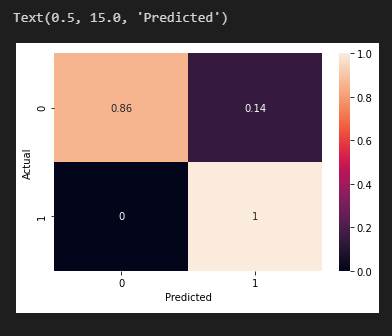
\includegraphics[width=0.7\linewidth]{Imagens/ConfusionMatrizNormalizado}
	\caption{86\% das entradas ruins foram classificadas como ruins e 100\% das boas foram classificadas como boas}
	\label{fig:confusionmatriznormalizado}
\end{figure}

 
\section{Mudança de configurações do modelo}

Para cada uma das seções a seguir, algum parâmetro do modelo será alterado, enquanto todos os outros serão mantidos iguais ao modelo criado na seção \ref{subsec:normalizada}, modelo cujos dados de entrada foram normalizados. O motivo de alterar apenas um parâmetro por vez é tornar mais clara a influência deste parâmetro na qualidade do modelo, uma vez que se alterássemos mais de um concomitantemente seria difícil distinguir qual mudança causou cada alteração nos resultados.

\subsection{Insira o conjunto de validação para o treinamento do modelo. Avalie o resultado obtido.}

Inserir o conjunto de validação para o treinamento do modelo significa separar parte dos dados de treino para a validação, de modo que esta parte separada não é utilizada durante o treinamento.

Ao inserir \textit{validation\_split=0.2} em nosso modelo, obtivemos os seguintes resultados. exibidos nas figuras abaixo.

\begin{figure}[H]
	\centering
	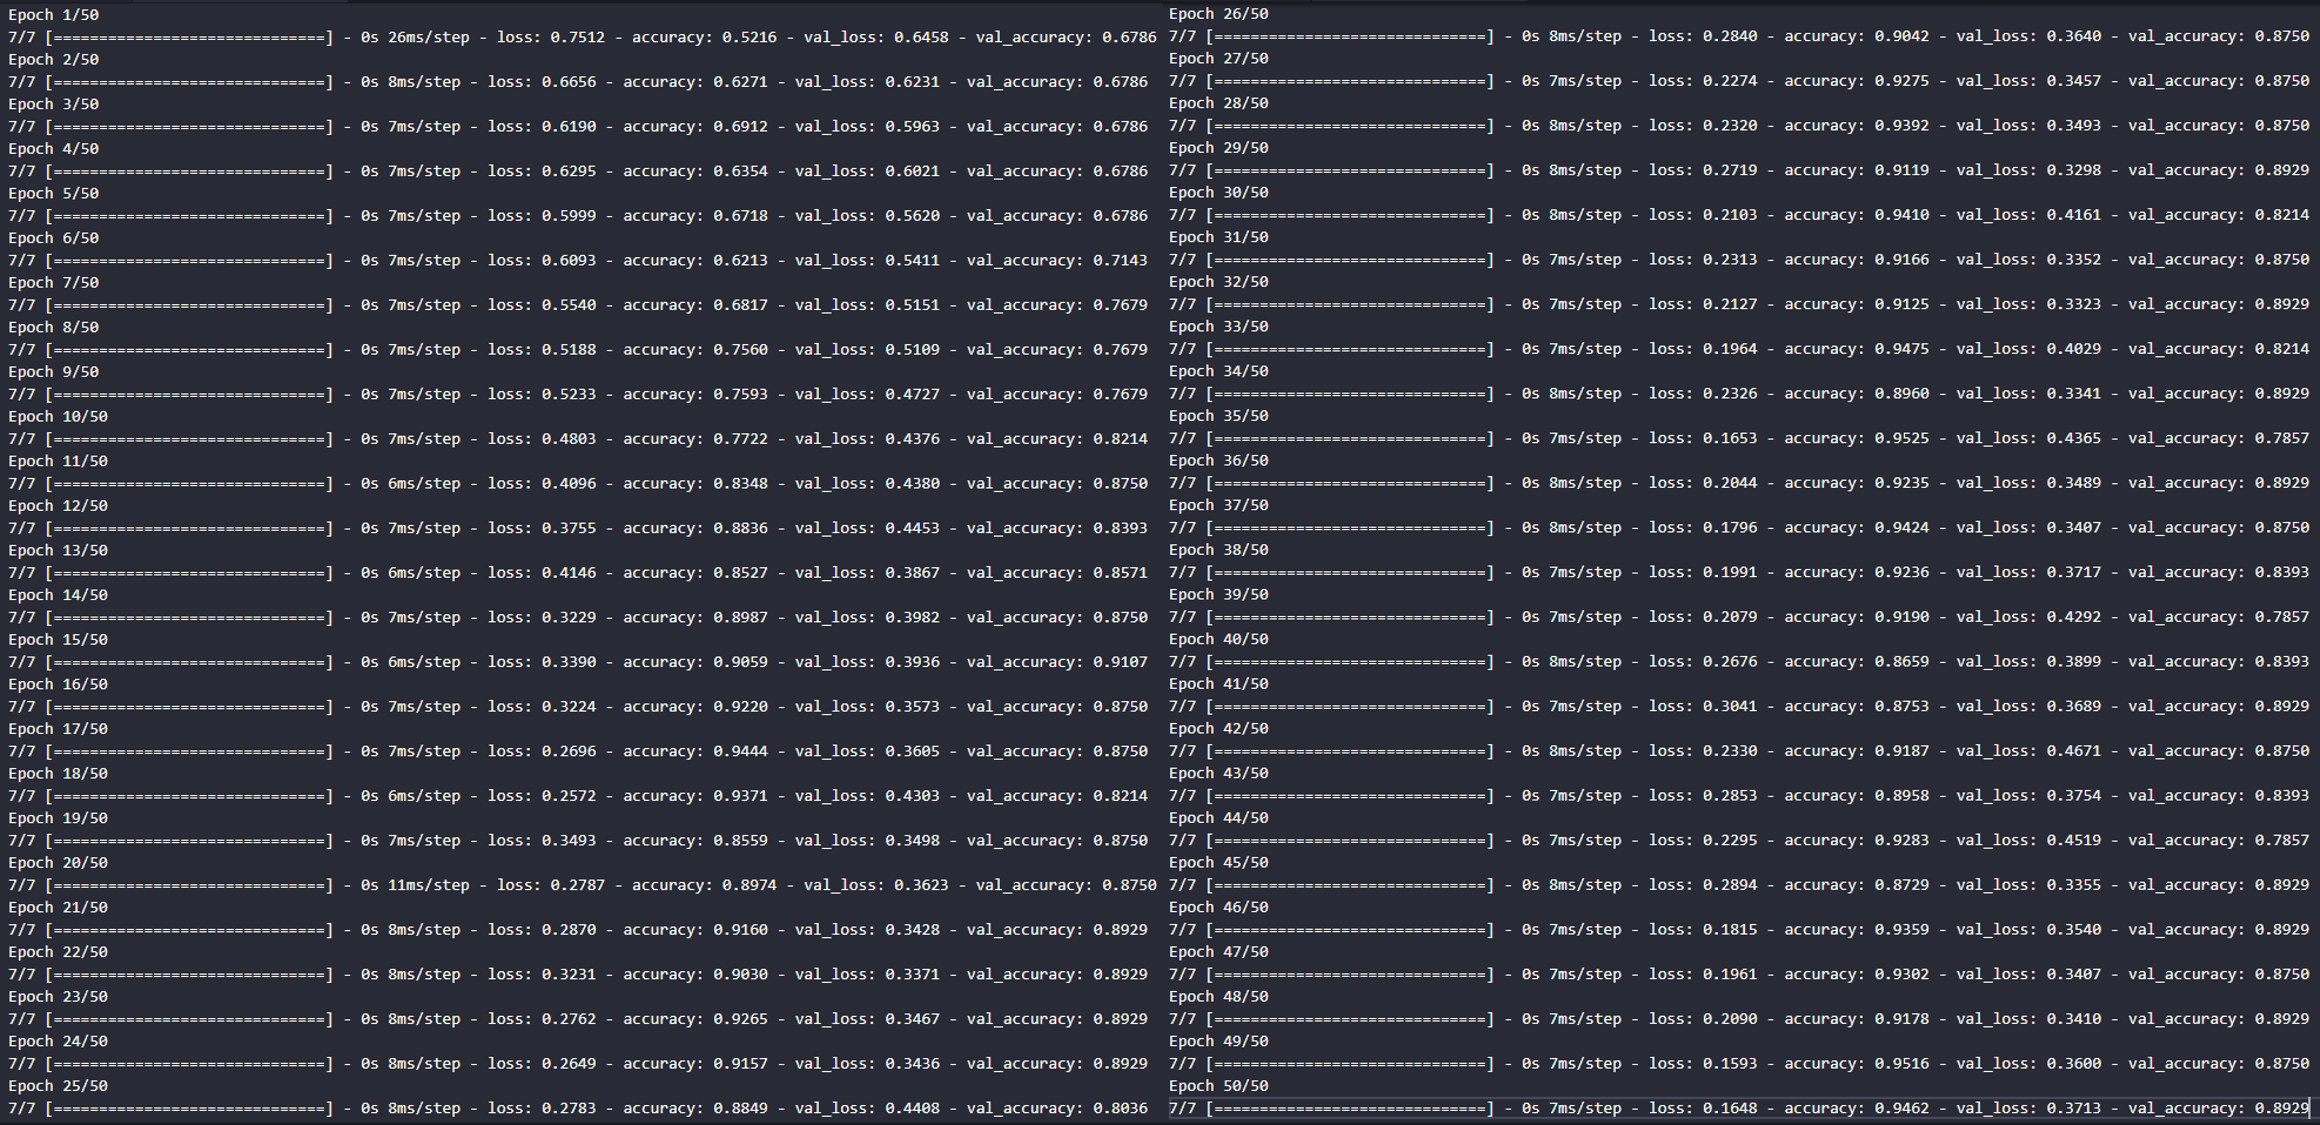
\includegraphics[width=1.1\linewidth]{Imagens/validacao/fitvalidacao}
	\caption{Retorno do treinamento com validation\_split=0.2}
	\label{fig:fitvalidacao}
\end{figure}
\begin{figure}[H]
	\centering
	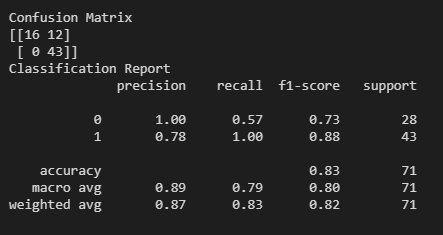
\includegraphics[width=0.7\linewidth]{Imagens/validacao/metricasvalidacao}
	\caption{Métricas do teste com validation\_split=0.2}
	\label{fig:metricasvalidacao}
\end{figure}
\begin{figure}[H]
	\centering
	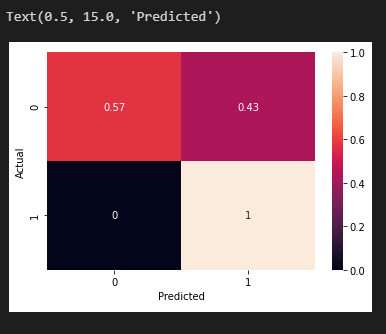
\includegraphics[width=0.7\linewidth]{Imagens/validacao/confusaovalidacao}
	\caption{Matriz de Confusão}
	\label{fig:confusaovalidacao}
\end{figure}
 
A priori, era de se esperar que separar um conjunto de dados para validação durante o treinamento melhorasse a qualidade da classificação da rede neural. No entanto, isso não parece ter acontecido.

A figura \ref{fig:metricasvalidacao} nos mostra uma acurácia de teste de 84\%, enquanto nossa rede original possuía acurácia de 94\%. Embora este resultado não seja o esperado, tentemos buscar uma explicação para ele.

O conjunto de validação presente poderia ajudar a verificar a ocorrência de \textit{overfitting}, mas a figura \ref{fig:fitvalidacao} não dá indícios que isso ocorreu. Podemos suspeitar desse fato uma vez que os valores de \textit{loss} e \textit{val\_loss} não apresentam perfil crescente em nenhum momento. O menor valor de \textit{loss} durante o treinamento é, aproximadamente, 0.16 e, de \textit{val\_loss}, 0.335. Os valores finais dessas métricas são similares aos mínimos. Logo, não parece ter ocorrido \textit{overfitting}.

Ao analisarmos a matriz de confusão da figura \ref{fig:confusaovalidacao}, bem como o recall da figura \ref{fig:metricasvalidacao}, notamos que a rede classificou corretamente todos os padrões de teste da classe 1 \textit{(good)}, mas apenas 57\% dos padrões da classe 0 \textit{(bad)}. Esta informação pode nos dar uma dica do porque desse modelo ser pior. Nossa base de dados é consideravelmente desbalanceada, com 225 padrões 1 e apenas 126 padrões 0. Sendo assim, ao retirarmos parte da base de dados do treinamento para a validação, a rede pode ter ficado com poucos padrões 0 para aprender, o que explicaria o péssimo rendimento na classificação dos padrões pertencentes a essa classe e, consequentemente, pioraria a qualidade da acurácia da rede.

\subsection{Modifique o tempo de treinamento (épocas) da Rede Neural. Escolha dois valores distintos (e.g. 1 e 1000 épocas) e avalie os resultados.}

Foram escolhidos os valores de 5 e de 1000 épocas para esta comparação. Esses valores, embora quase arbitrários, possuem uma motivação de escolha. Como na seção \ref{subsec:normalizada}, com 50 épocas, o resultado da rede foi bom, vamos observar o que acontece com a qualidade do modelo quando ele é pouquíssimo treinado e quando ele é super-treinado. Podemos suspeitar que veremos um \textit{underfitting} e um \textit{overfitting} de nosso modelo. Vejamos os resultados. 

\subsubsection{5 épocas}

As figuras abaixo ilustram o output do treinamento do modelo, as métricas analisadas e a matriz de confusão, respectivamente, do modelo com 5 épocas apenas.

\begin{figure}[H]
	\centering
	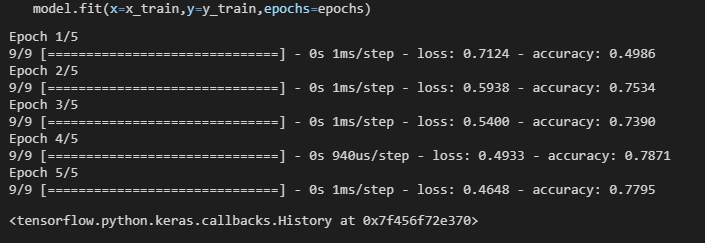
\includegraphics[width=0.7\linewidth]{Imagens/5epocas/fit5epocas}
	\caption{Output do treinamento do modelo com 5 épocas}
	\label{fig:fit5epocas}
\end{figure}
\begin{figure}[H]
	\centering
	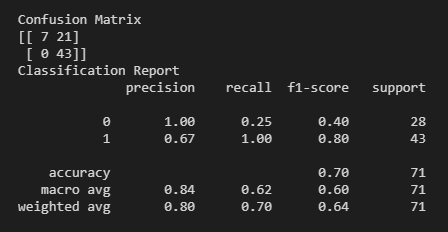
\includegraphics[width=0.7\linewidth]{Imagens/5epocas/metricas5epocas}
	\caption{Métricas do modelo com 5 épocas}
	\label{fig:metricas5epocas}
\end{figure}
\begin{figure}[H]
	\centering
	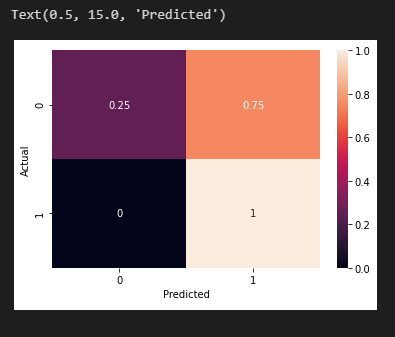
\includegraphics[width=0.7\linewidth]{Imagens/5epocas/confusao5epocas}
	\caption{Matriz de Confusão do modelo com 5 épocas}
	\label{fig:confusao5epocas}
\end{figure}

Analisando a figura \ref{fig:fit5epocas} podemos, rapidamente, perceber que a acurácia de nosso modelo ao longo do treinamento não passou dos 78\%. Se analisarmos esta imagem em conjunto com a figura \ref{fig:fitnormalizada} que mostrava esta mesma informação para 50 épocas, notamos que no caso anterior precisamos de mais de 5 épocas para a acurácia atingir valores decentes. 

Ao analisarmos a acurácia na figura \ref{fig:metricas5epocas} vemos que ela é muito menor do que a obtida com 50 épocas. Isso está relacionado com o que foi discutido no parágrafo anterior. Mais especificamente, podemos comentar o seguinte: nosso modelo possui 526 parâmetros treináveis e as 5 épocas não foram suficientes para treiná-los de modo a tornar esta rede satisfatoriamente especializada. Aqui percebemos um problema de \textit{underfitting} pois nossa rede não foi capaz de aprender todos os padrões do conjunto de treinamento. As demais métricas devem corroborar com esta conclusão. Vejamos.

A precisão deste modelo é interessante. Embora nossa acurácia tenha sido ruim, a rede possui precisão de 100\% para a classe "bad" (0), embora apenas 67\% para a classe "good" (1).

O recall, de forma similar, apresenta 100\% para a classe "good" e apenas 25\% para a classe "bad". O motivo para o recall da classe 0 ser tão ruim, pode ser o fato de haver poucos padrões classificados como "bad" para o treinamento. Isso, somado com as pouquíssimas épocas, pode ter feito este modelo não aprender a classificar corretamente padrões desta classe.

O f1-score resultante foi 40\% para a classe "bad" e 80\% para a classe "good". Analisando apenas o comportamento da precisão e do recall deste modelo em relação ao modelo de 50 épocas, poderíamos ficar em dúvida sobre o fato dele ser pior ou melhor com base nessas métricas. No entanto, o f1-score, por ser uma análise conjunta da precisão e recall, deixa claro o pior rendimento desta rede em relação à anterior, uma vez que, para ambas as classes, o valor é menor.

Com isso, podemos argumentar fortemente que o modelo não foi treinado o suficiente e não convergiu para a função desejada.


\subsubsection{1000 épocas}

As figuras abaixo ilustram as métricas analisadas e a matriz de confusão, respectivamente, do modelo com 1000 épocas. O output do treinamento não foi incluído por ser grande demais para este relatório, mas pode ser consultado no notebook enviado em conjunto com este documento.

\begin{figure}[H]
	\centering
	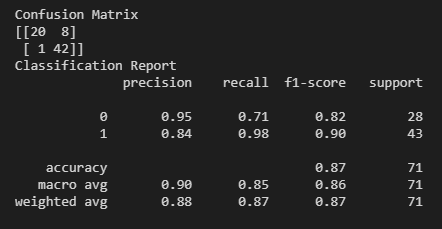
\includegraphics[width=0.7\linewidth]{Imagens/1000epocas/metricas1000epocas}
	\caption{Métricas do modelo com 1000 épocas}
	\label{fig:metricas1000epocas}
\end{figure}
\begin{figure}[H]
	\centering
	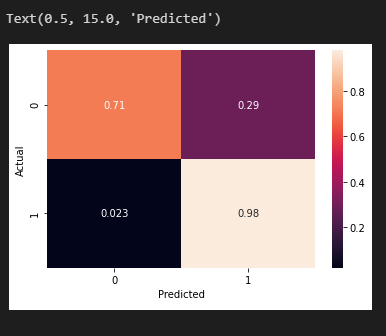
\includegraphics[width=0.7\linewidth]{Imagens/1000epocas/confusao1000epocas}
	\caption{Matriz de Confusão do modelo com 1000 épocas}
	\label{fig:confusao1000epocas}
\end{figure}

Ao analisar o output do treinamento, que não está exibido neste relatório, percebemos pouca diferença na acurácia e na função de perda do modelo, em relação à 50 épocas. Vale comentar apenas que os valores da acurácia deste output são todos muito bons, com a grande maioria acima de 95\%. No entanto, veremos que isso não implica, necessariamente, em uma rede adequada.

Ao analisar a acurácia geral deste modelo notamos uma queda, uma vez que seu valor é de 87\%. Essa diferença entre a acurácia geral e acurácia durante o treinamento pode ser sinal de uma superespecialização da rede, que praticamente "decorou" os padrões de treino e criou uma função excessivamente flexível, que perde generalização. Como temos apenas 526 pesos, estabelecer 1000 épocas parece se mostrar exagerado para o treinamento. Isso explica a acurácia excelente durante o treinamento, mas baixa no teste. 

Ao analisarmos as demais métricas exibidas na figura \ref{fig:confusao1000epocas} e comparar com as métricas da rede com 50 épocas percebemos uma piora em todos os valores. No entanto, a evolução da métrica \textit{loss} não revela nenhum padrão crescente, permanecendo sempre abaixo de 0.1, o que corrobora para a argumentação que esta rede, embora treinada demais, não sofre um \textit{overfitting}. Sendo assim, considera-se inconclusiva a existência ou não de \textit{overfitting}.

\subsection{Modifique a taxa de aprendizado da Rede Neural. Escolha dois valores distintos (e.g. 0,001 e 0,1) e avalie os resultados.}

A taxa de aprendizado de uma Rede Neural está relacionada com a a velocidade na qual a rede treina, com o problema dos mínimos locais e com possíveis oscilações no treinamento da rede. Caso a taxa seja muito pequena, nosso treinamento será mais lento e corremos maiores riscos de convergir para um mínimo local, ao invés de atingir o mínimo global da função de erro do modelo. Isso, obviamente, é indesejado, pois queremos o menor erro possível para a rede modelada. Caso a taxa seja grande demais, por outro lado, corremos o risco de ficar oscilando no entorno de um mínimo da função de erro, uma vez que os "saltos" de nossa rede são grandes demais. Veremos como esses conceitos aparecem na análise da rede neural com taxas de aprendizado 0.001 e 0.4, lembrando que, originalmente, a taxa valia 0.05. Novamente, esses valores foram escolhidos por serem muito menor e muito maior que o valor original, para o qual a rede demonstrou bom desempenho.

\subsubsection{Taxa de aprendizado = 0.001}

As figuras abaixo ilustram o retorno do treinamento da rede, as métricas analisadas e a matriz de confusão, respectivamente, do modelo com taxa de aprendizado igual a 0.001. 

\begin{figure}[H]
	\centering
	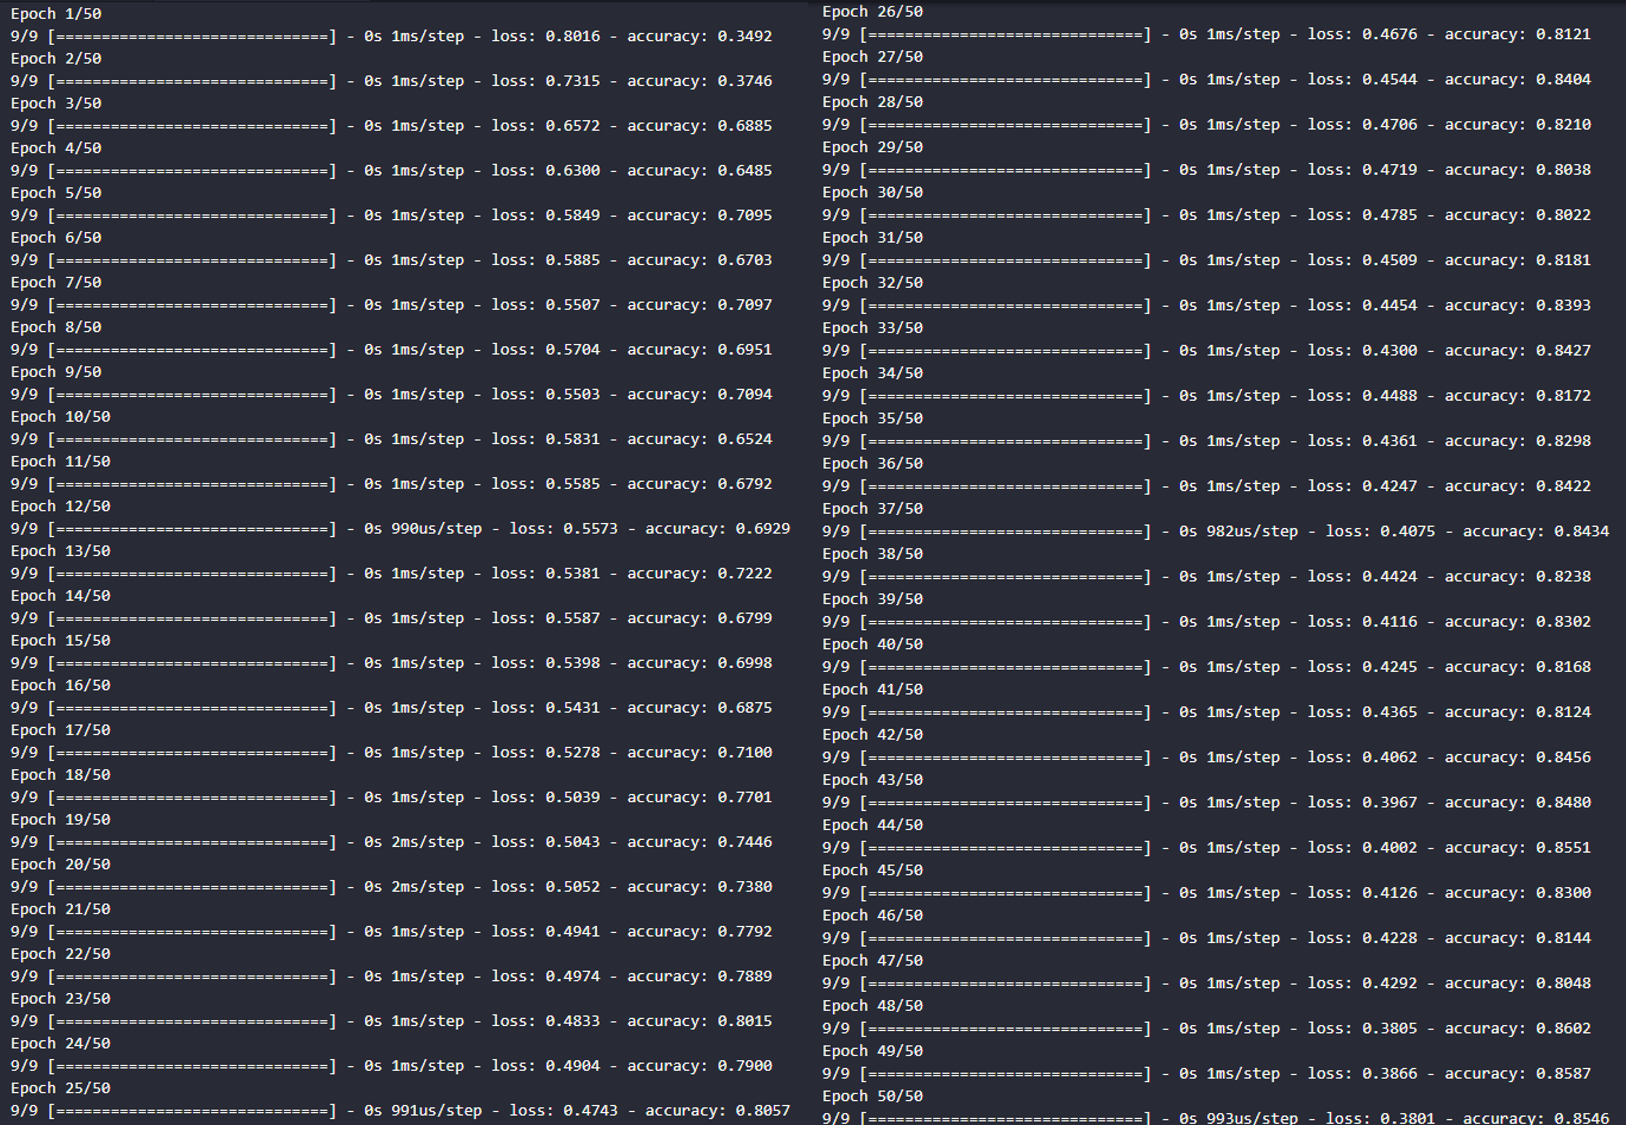
\includegraphics[width=1.1\linewidth]{Imagens/taxa0001/fittaxa0001}
	\caption{Treinamento da rede neural com taxa de aprendizado 0.001}
	\label{fig:fittaxa0001}
\end{figure}
\begin{figure}[H]
	\centering
	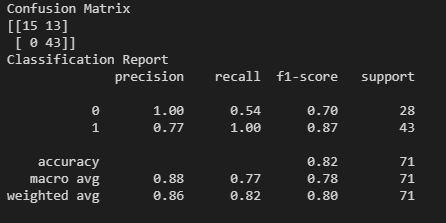
\includegraphics[width=0.7\linewidth]{Imagens/taxa0001/metricastaxa0001}
	\caption{Métricas para taxa de aprendizado 0.001}
	\label{fig:metricastaxa0001}
\end{figure}
\begin{figure}[H]
	\centering
	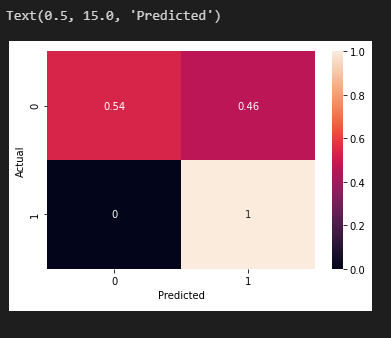
\includegraphics[width=0.7\linewidth]{Imagens/taxa0001/confusaotaxa0001}
	\caption{Matriz de Confusão para taxa de aprendizado 0.001}
	\label{fig:confusaotaxa0001}
\end{figure}

Ao analisar a figura \ref{fig:fittaxa0001}, uma informação que se destaca é o campo \textit{loss}. Este campo é o erro que queremos minimizar com o treinamento de rede. Com isso em mente, note que os valores de \textit{loss} para esta taxa de aprendizado estão consideravelmente maiores em relação ao modelo com taxa 0.05. Naquele, a perda era minimizada até 0.11, enquanto aqui ela pouca abaixa de 0.4. Esse fato é um grande indicador que a taxa escolhida pode ter sido pequena demais, o que revela que talvez a rede tenha convergido para um mínimo local da função de erro. A acurácia exibida nesta mesma figura também é pior que aquela apresentada com a taxa original, e a acurácia dos testes, exibida na figura \ref{fig:metricastaxa0001} é de 82\%, menor que a original.

A precisão para a classe "bad" e o recall para a classe "good" apresentam os mesmos valores para a taxa de aprendizado original, ambos 1.0. Entretanto, a precisão da classe "good" e o "recall" da classe "bad" são ambos piores que os originais. Mais uma vez, utilizemos o f1-score para averiguar que a média das métricas anteriores é pior, para ambas as classes, em relação ao modelo original. Essas análises, somadas com o que foi comentado sobre a perda grande do modelo, atestam para o fato de que esta rede é menos adequada que a original. 
\subsubsection{Taxa de aprendizado = 0.4}

As figuras abaixo ilustram o retorno do treinamento da rede, as métricas analisadas e a matriz de confusão, respectivamente, do modelo com taxa de aprendizado igual a 0.4. 

\begin{figure}[H]
	\centering
	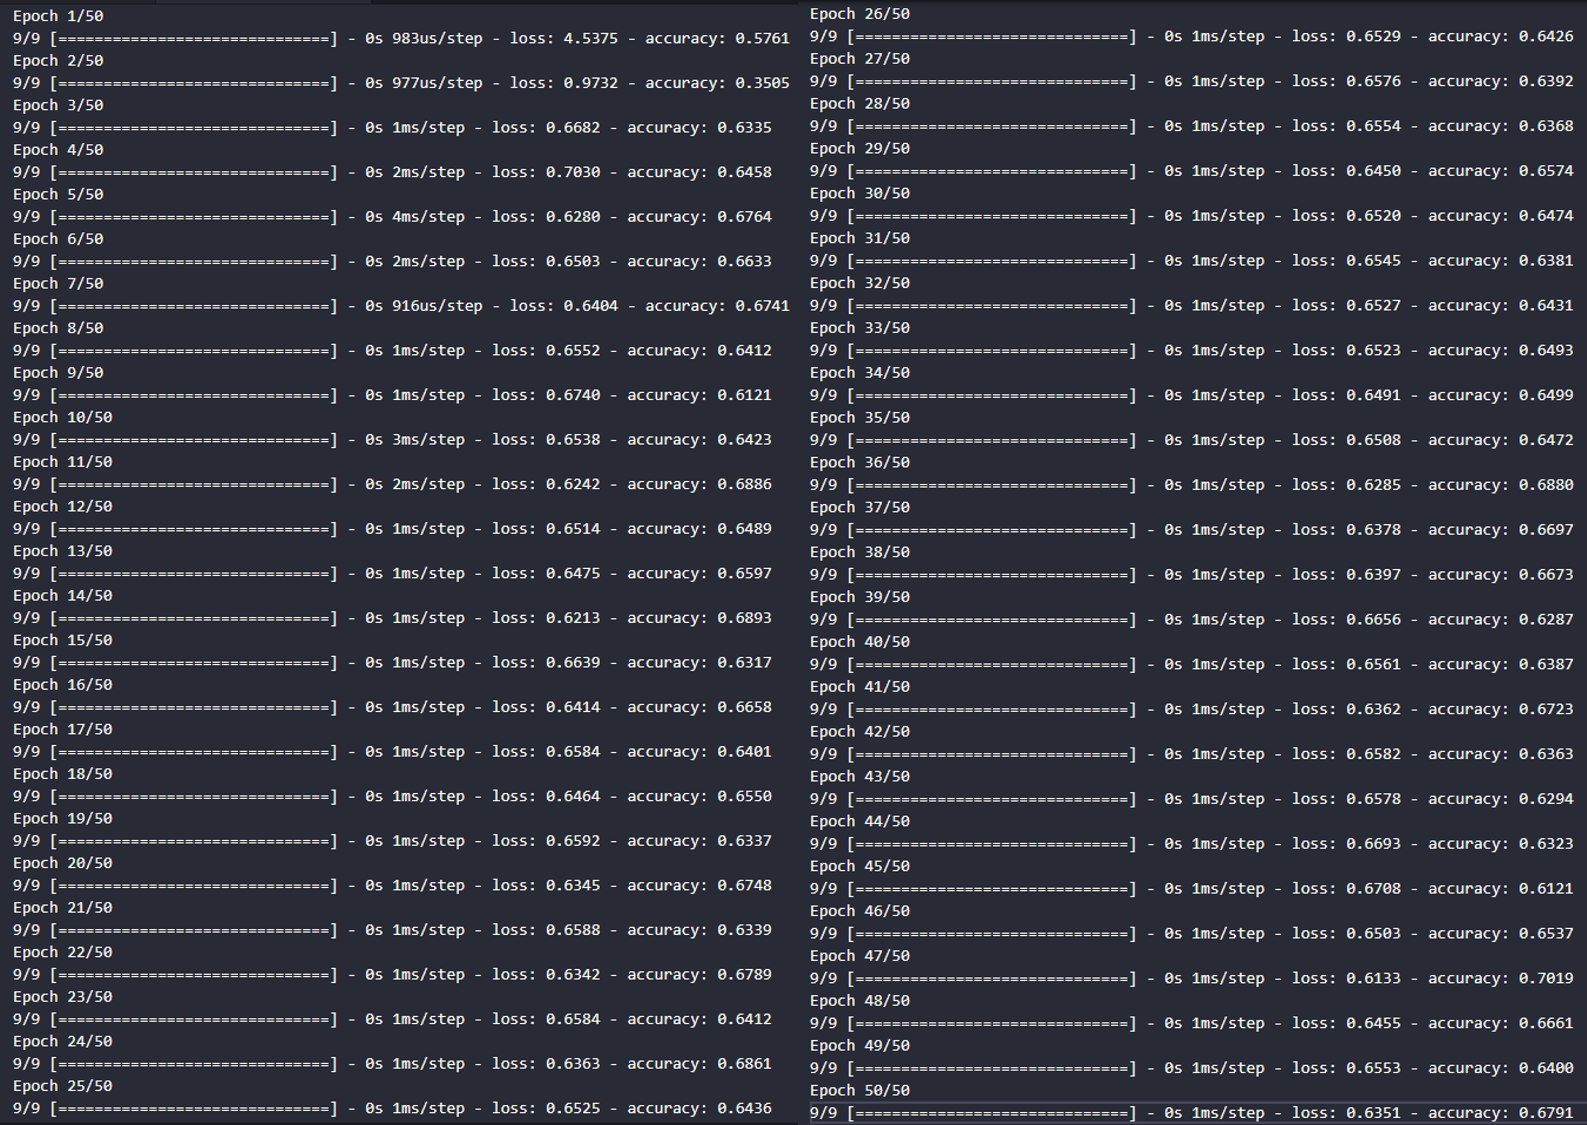
\includegraphics[width=1.1\linewidth]{Imagens/taxa04/fittaxa04}
	\caption{Treinamento da rede neural com taxa de aprendizado 0.4}
	\label{fig:fittaxa04}
\end{figure}
\begin{figure}[H]
	\centering
	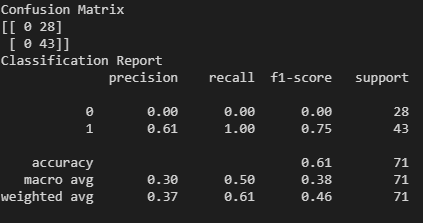
\includegraphics[width=0.7\linewidth]{Imagens/taxa04/metricastaxa04}
	\caption{Métricas para taxa de aprendizado 0.4}
	\label{fig:metricastaxa04}
\end{figure}
\begin{figure}[H]
	\centering
	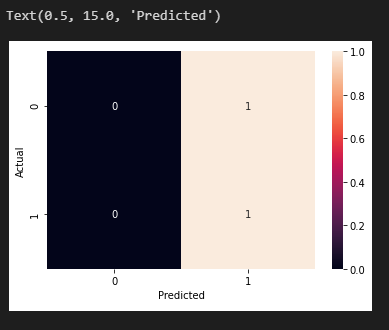
\includegraphics[width=0.7\linewidth]{Imagens/taxa04/confusaotaxa04}
	\caption{Matriz de Confusão para taxa de aprendizado 0.4}
	\label{fig:confusaotaxa04}
\end{figure}

Vamos, novamente, começar analisando a perda do treinamento. Note que, logo a partir da quinta época, o valor de \textit{loss} parece ficar sempre próximo a 0.64, indo de aproximadamente 0.62 até 0.67. Isso mostra, justamente, um perfil de oscilação da minimização do valor do erro da rede. Há uma diferença entre esta oscilação visível na figura \ref{fig:fittaxa04} e a convergência para um minimo local apresentada na figura \ref{fig:fittaxa0001}. Lá os valores de erro decresceram ao longo do treinamento e convergiram para um valor ruim. Aqui não há minimização, ou, pelo menos, há pouca, o que indica a oscilação já comentada. Esse fato é indicador de que a nossa taxa de aprendizagem, 0.4, é grande demais. As demais métricas, provavelmente, darão outros indícios da má qualidade do modelo.

A acurácia do teste, exibida na figura \ref{fig:metricastaxa04} foi a pior de todas até agora, 0.61. Além disso, a figura \ref{fig:confusaotaxa04} nos mostra que todos os dados de teste da classe 0 foram erroneamente classificados como 1 e todos os dados de teste da classe 1 foram corretamente classificados. Estes valores de precisão, recall e f1-score nos mostram que este rede não é confiável para fazer a classificação que buscamos. 

\subsection{Modifique a quantidade de neurônios na camada escondida da Rede Neural. Escolha dois valores distintos (e.g. 2 e 70 neurônios) e avalie os	resultados.}

O número de neurônios da camada escondida está diretamente relacionado com a quantidade de pesos que nosso modelo deverá treinar. Como cada neurônio está conectado com todas as entradas e com a saída, e cada conexão possui um peso, além dos \textit{bias} de cada neurônio, uma rede neural com muitos neurônios na camada escondida pode se tornar custosa e complexa desnecessariamente. Foram escolhidos os valores 5 e 50 por, mais uma vez, serem bem menor e maior que o original.

\subsubsection{5 neurônios}

As figuras abaixo ilustram o sumário da rede, o retorno do treinamento da rede, as métricas analisadas e a matriz de confusão, respectivamente, do modelo com 5 neurônios na camada escondida. A figura \ref{fig:sumario5neuronios} mostra que, neste caso, temos 176 parâmetros para treinar.

\begin{figure}[H]
	\centering
	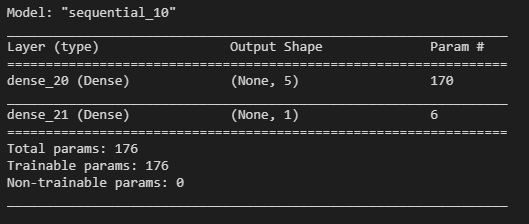
\includegraphics[width=0.7\linewidth]{Imagens/5neuronios/sumario5neuronios}
	\caption{Sumário do modelo com 5 neurônios na camada escondida}
	\label{fig:sumario5neuronios}
\end{figure}
\begin{figure}[H]
	\centering
	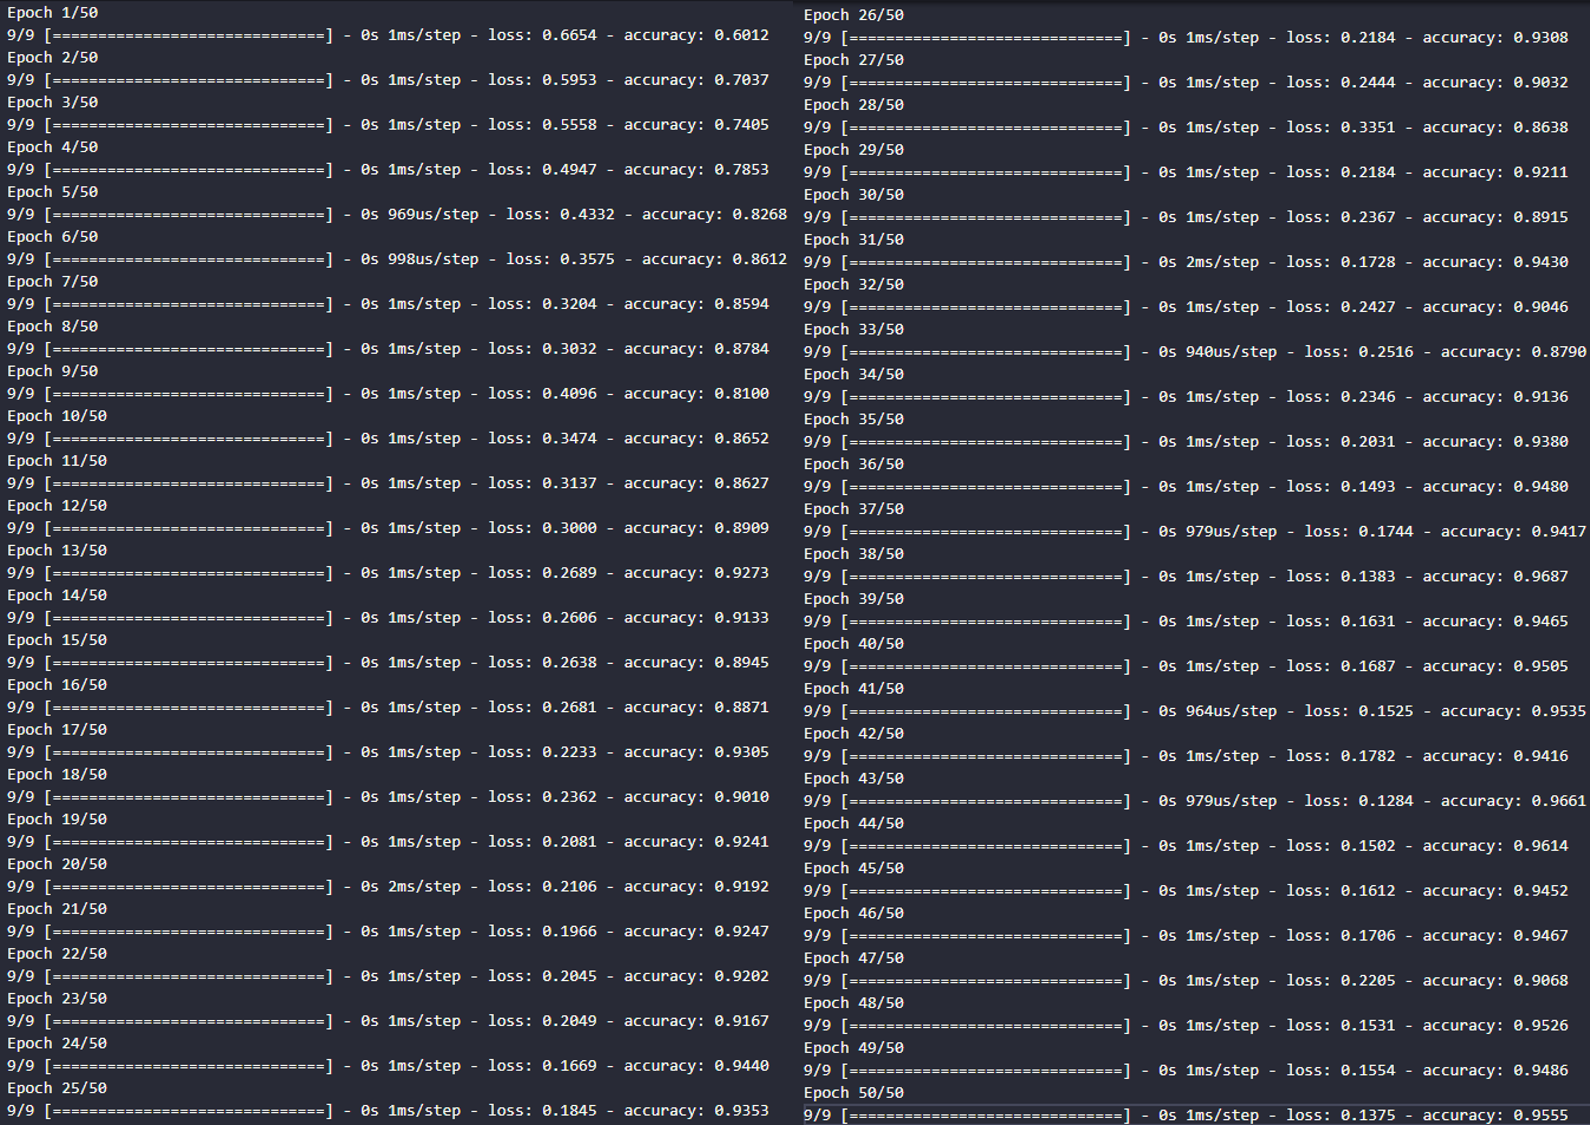
\includegraphics[width=1.1\linewidth]{Imagens/5neuronios/fit5neuronios}
	\caption{Treinamento do modelo com 5 neurônios na camada escondida}
	\label{fig:fit5neuronios}
\end{figure}
\begin{figure}[H]
	\centering
	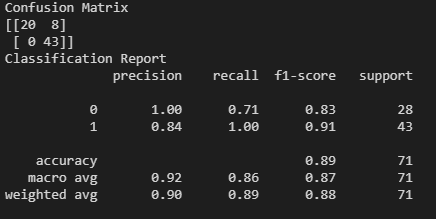
\includegraphics[width=0.7\linewidth]{Imagens/5neuronios/metricas5neuronios}
	\caption{Métricas do modelo com 5 neurônios na camada escondida}
	\label{fig:metricas5neuronios}
\end{figure}
\begin{figure}[H]
	\centering
	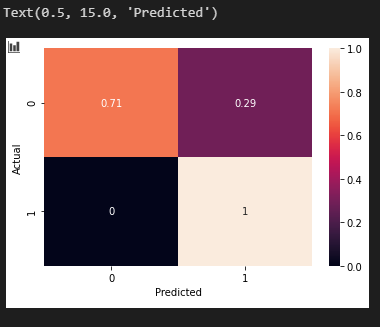
\includegraphics[width=0.7\linewidth]{Imagens/5neuronios/confusao5neuronios}
	\caption{Matriz de Confusão do modelo com 5 neurônios na camada escondida}
	\label{fig:confusao5neuronios}
\end{figure}

Ao analisarmos a evolução da acurácia e da perda na figura \ref{fig:fit5neuronios} não percebemos grandes diferenças em relação ao modelo original. Isso pode indicar que ambas as quantidades de neurônios são razoáveis para este problema de classificação. Analisemos as demais métricas para averiguar se este fato é verídico.

A acurácia dos testes, 89\% foi menor que a apresentada pela rede original. A precisão para a classe 0 e o recall para a classe 1 foram iguais aos do modelo original, enquanto que a precisão da classe 1 e o recall da classe 0 foram um pouco menores. Com base nisso, não é de espantar que o f1-score é um pouco menor para ambas as classes. Todos esses valores estão apresentados na figura \ref{fig:metricas5neuronios}. Sendo assim, em comparação à rede com 15 neurônios, esta rede com 5 não apresentou uma perda enorme em qualidade, apesar de se mostrar pior. Vejamos o que ocorre ao aumentar o número de neurônios da camada escondida.

\subsubsection{50 neurônios}

As figuras abaixo ilustram o sumário da rede, o retorno do treinamento da rede, as métricas analisadas e a matriz de confusão, respectivamente, do modelo com 50 neurônios na camada escondida. A figura \ref{fig:sumario50neuronios} mostra que, neste caso, temos 1751 parâmetros para treinar.

\begin{figure}[H]
	\centering
	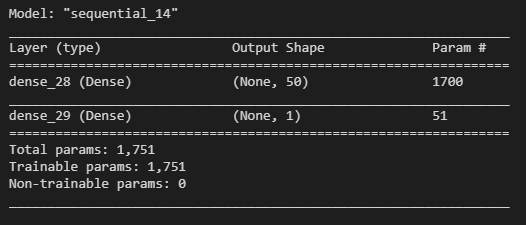
\includegraphics[width=0.7\linewidth]{Imagens/50neuronios/sumario50neuronios}
	\caption{Sumário do modelo com 50 neurônios na camada escondida}
	\label{fig:sumario50neuronios}
\end{figure}
\begin{figure}[H]
	\centering
	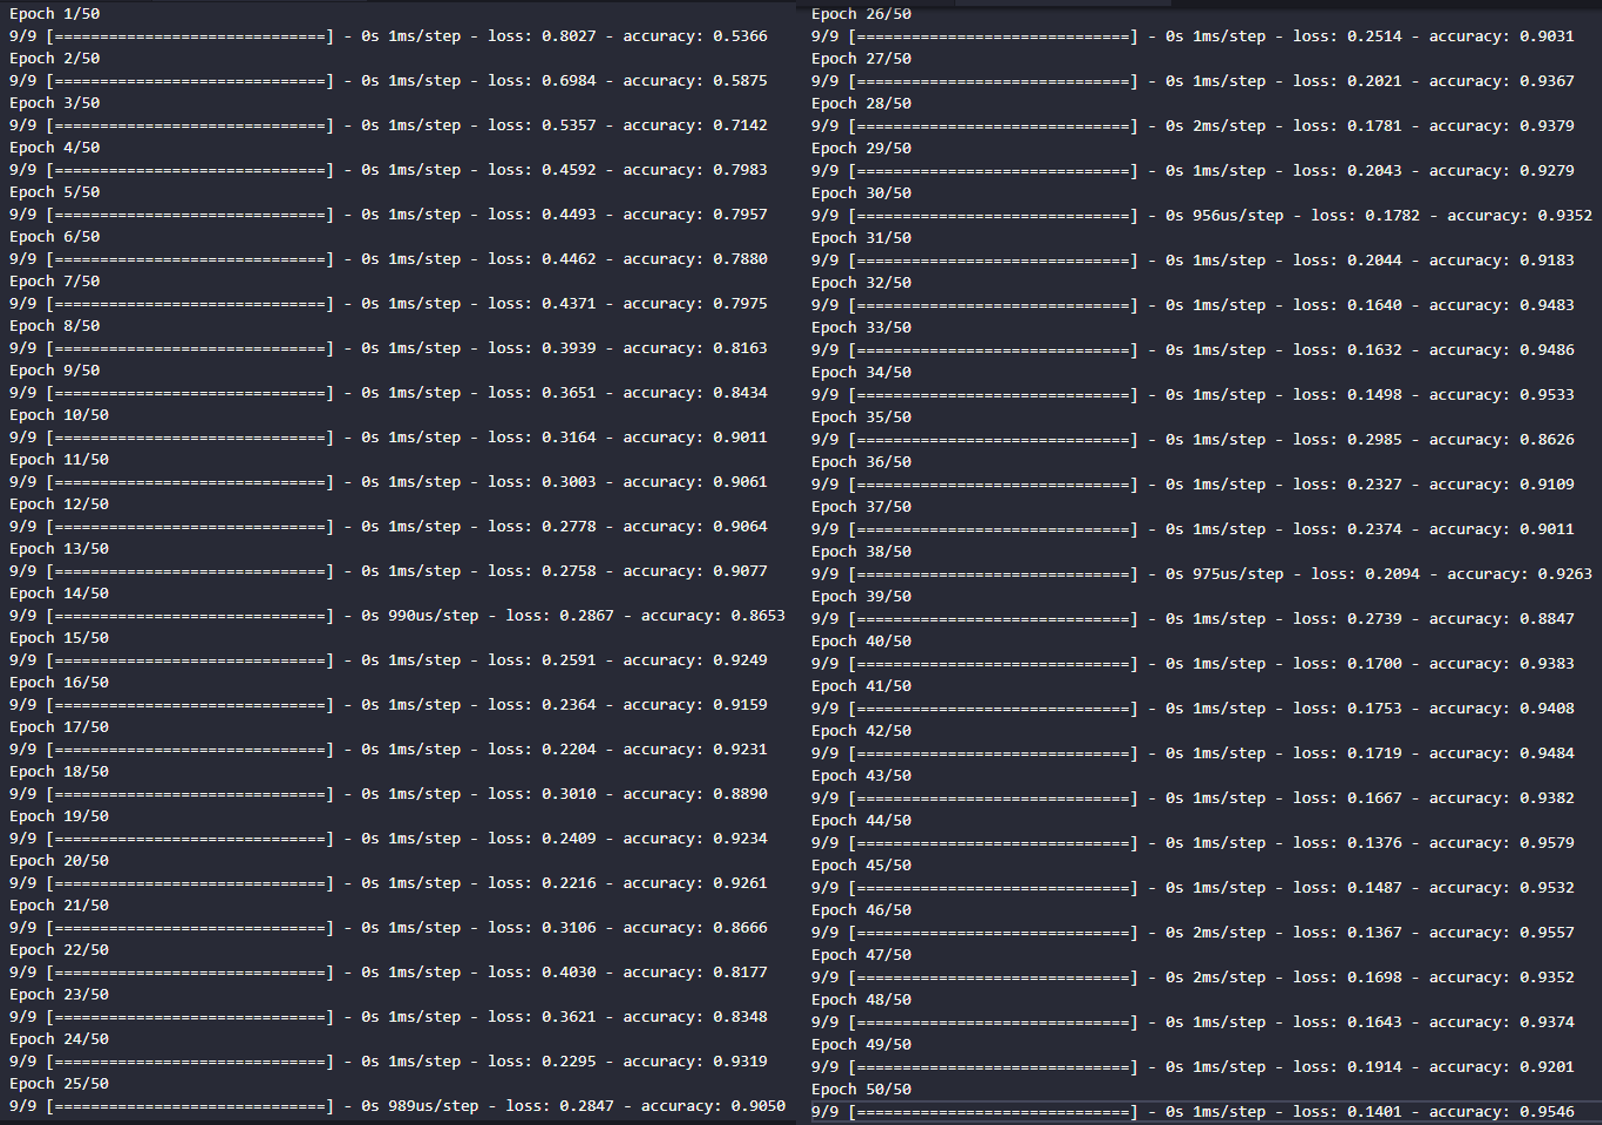
\includegraphics[width=1.1\linewidth]{Imagens/50neuronios/fit50neuronios}
	\caption{Treinamento do modelo com 50 neurônios na camada escondida}
	\label{fig:fit50neuronios}
\end{figure}
\begin{figure}[H]
	\centering
	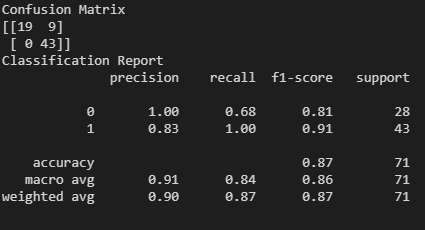
\includegraphics[width=0.7\linewidth]{Imagens/50neuronios/metricas50neuronios}
	\caption{Métricas do modelo com 50 neurônios na camada escondida}
	\label{fig:metricas50neuronios}
\end{figure}
\begin{figure}[H]
	\centering
	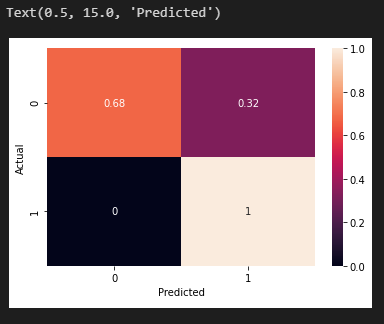
\includegraphics[width=0.7\linewidth]{Imagens/50neuronios/confusao50neuronios}
	\caption{Matriz de Confusão do modelo com 50 neurônios na camada escondida}
	\label{fig:confusao50neuronios}
\end{figure}

Curiosamente, todas as métricas são bastante similares em relação ao modelo com 5 neurônios apenas, e ainda piores que as métricas apresentadas pelo modelo original. Isso nos indica que, para este problema de classificação da base de dados Ionosphere, a quantidade de neurônios não influencia muito na qualidade da rede criada. Mais que isso, parece que a quantidade ótima de neurônios pode estar próxima da quantidade utilizada no modelo original, 15, uma vez que, tanto ao aumentar quanto ao diminuir este parâmetro, a rede piorou. 
\section{Teste Livre}\label{sec:testelivre}

\subsection{Faça novos testes para avaliar o desempenho da Rede Neural no	problema designado. Use a técnica K-Fold (com K = 10) para analisar o	resultado obtido.}

A técnica K-Fold Validation consiste em separa a base de dados em $K$ grupos, sendo que $K-1$ desses grupos são usados para treinamento enquanto o grupo restante é usado para teste. O processo de treinamento é realizado $K$ vezes, até que todos os grupos tenham sido usados para teste.A performance global de cada topologia é calculada como a média de cada performance individual para cada $K$ treino. \cite{Livro} 

Ao utilizar essa técnica pela primeira vez, um erro surgiu. Como a base de dados Ionosphere é razoavelmente desbalanceada e os últimos padrões de entrada, como dispostos no arquivo disponibilizado, são da classe "good", ao separar os 10 grupos, houve grupos sem nenhum padrão da classe "bad". Isso foi resolvido utilizando o parâmetro \textit{shuffle=True} para embaralhar ao invés de selecionar os grupos sequencialmente.

As figuras abaixo exibem as métricas e a matriz de confusão.

\begin{figure}[H]
	\centering
	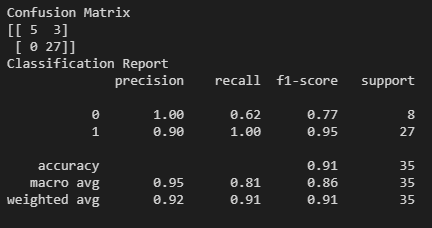
\includegraphics[width=0.7\linewidth]{Imagens/metricasconfusao}
	\caption{Métricas do modelo com K-Fold com $k=10$}
	\label{fig:metricasconfusao}
\end{figure}
\begin{figure}[H]
	\centering
	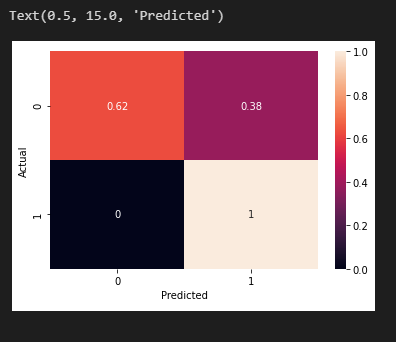
\includegraphics[width=0.7\linewidth]{Imagens/kfoldconfusao}
	\caption{Matriz de Confusão do modelo com K-Fold com $k=10$}
	\label{fig:kfoldconfusao}
\end{figure}

Nota-se que a acurácia geral do modelo foi de 91\% e que, fora a Rede Original, é a melhor acurácia obtida no trabalho. As métricas precisão e recall também possuem valores similares que os obtidos com a rede original, embora o recall e f1-score da classe "bad" seja pior. Provavelmente, o motivo para isso é, novamente, o fato de haver poucos padrões dessa classe para treinamento, em relação aos da classe "good". Perceba que apenas 8 padrões da classe 0 foram usados para teste.

Mesmo com o desbalanceamento da base de dados, essa técnica se mostrou com o melhor resultado dentre todas as alterações realizadas em cada seção deste relatório.

\subsection{Faça análises e novas implementações que você julgue importante para o seu trabalho. Não esqueça de explicar a motivação da análise realizada.}

\subsubsection{Early Stopping}

O intuito de implementar o \textit{early stopping} é, simplesmente, aprender a usá-lo na prática, analisando seus parâmetros e impactos na qualidade da rede. Alguns testes foram realizados antes do modelo exibido neste relatório com o intuito de estudar a implementação e ver como a alteração de cada parâmetro impactou a classificação. Entre esses parâmetros, foram variados a épocas (valores de 50 e 70) e o número de neurônios na camada escondida (15 e 20).

Para o \textit{EarlyStopping} foi definido um \textit{callback} com \textit{monitor='accuracy'} e \textit{patience=10}. Isso quer dizer que, se a métrica acurácia não exibir nenhum aumento em seu valor em 10 épocas, a rede para de treinar e fica com os pesos deste momento. Essa é uma estratégia para, no caso de muitas épocas (estamos com 70), evitar o \textit{overfitting}, pois, uma vez que em 10 épocas a acurácia não aumentou, é provável que não aumente mais e nossa rede apenas perca generalização com os treinos faltantes.

A figura \ref{fig:fitearly} exibe exatamente isso: a acurácia na época 26 foi de 0.9737 e após 10 épocas, nenhuma acurácia foi maior que ela, o que resultou na parada do treinamento na época 36.
\begin{figure}[H]
	\centering
	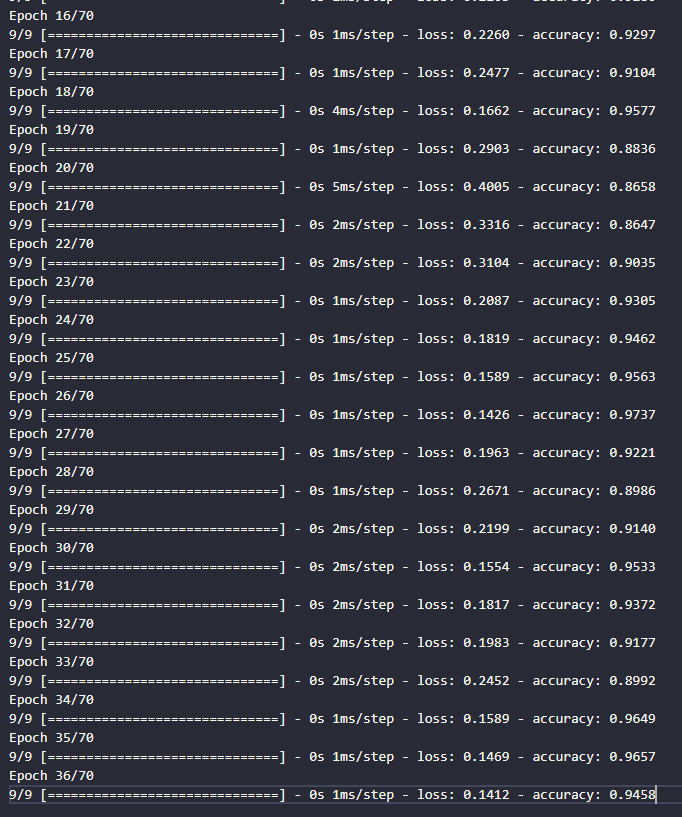
\includegraphics[width=0.7\linewidth]{Imagens/earlystopping/fitearly}
	\caption{Treinamento do modelo com early stopping}
	\label{fig:fitearly}
\end{figure}

Embora a minha ideia tenha sido evitar um \textit{overfitting}, parece que o problema contrário ocorreu. Como pode ser visto na figura \ref{fig:metricasearly}, a acurácia geral do modelo foi de apenas 0.85, bem menor que a original. Isso pode indicar que, ao parar na época 36 a rede ainda não havia treinado o suficiente seus pesos. O f1-score também ser menor corrobora com esta possibilidade.

Sendo assim, utilizar o \textit{EarlyStopping} requer maiores estudos e testes para a escolha correta de todos os parâmetros da rede, visto que apenas abortar o treinamento ao perceber a falta de evolução em alguma métrica após $p$ épocas não significa, necessariamente, que tal métrica não voltará a evoluir positivamente na época $p+1$.
\begin{figure}[H]
	\centering
	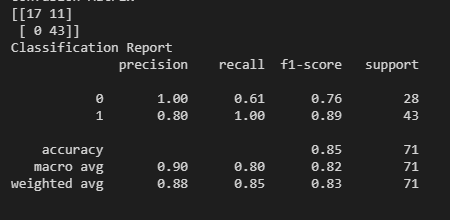
\includegraphics[width=0.7\linewidth]{Imagens/earlystopping/metricasearly}
	\caption{Métricas do teste com EarlyStopping}
	\label{fig:metricasearly}
\end{figure}



\begin{thebibliography}{99} 
	
	\bibitem{Dataset} 
	UCI Machine Learning Repository,\\ \texttt{https://archive.ics.uci.edu/ml/datasets/Ionosphere}
	
	\bibitem{Paper1989} Sigillito, V. G., Wing, S. P., Hutton, L. V., \& Baker, K. B. (1989). \textit{Classification of radar returns from the ionosphere using neural networks.} Johns Hopkins APL Technical Digest, 10, 262-266.
	
	\bibitem{Livro} Ivan Nunes da Silva, Danilo Hernane Spatti, Rogério Andrade Flauzino, \textit{}Redes Neurais Artificiais para Engenharia e Ciências
	Aplicadas: Curso Prático, Artliber Editora, 2010.
	
	
	
	
\end{thebibliography}
\end{document}